Dans cette partie, nous allons traiter des différentes fonctionnalités présentées par la solution. Nous aborderons tant le point de vue des applications utilisatrices de ce service, que le point de vue de la gestion du service.

\subsubsection{Concepts introduits}

Avant de présenter les diverses fonctionnalités, certains mécanismes visant à la qualité du service vont être présentés.

Pour commencer, un service de \underline{DNS} est utilisé. Ce type de service permet d'attribuer une URL textuelle à un adresse IP (l'adresse du serveur web). Ainsi, les utilisateurs retiendront plus facilement cette URL plutôt que l'adresse IP, et cela permet de configurer les applications clientes plus facilement (en renseignant simplement l'URL textuelle).

De plus, il faut noter que dans certains cas, l'adresse IP d'un serveur n'est pas attribuée de manière statique. Pour remédier à cela, nous avons ajouté un service \underline{DynDNS}. Ce service va mettre en place un mécanisme mettant à jour l'adresse IP à associer à l'URL textuelle définie avec le DNS. De ce fait, il n'y a plus besoin de s'occuper des changements dynamiques d'IP du serveur web. Grâce à cela, nous pourrons toujours accéder au service à l'aide de l'URL \textbf{https://watchdogzz.ddns.net}.

Comme nous pouvons le constater dans l'URL fournie précédement, nous utilisons le protocole \textbf{\underline{https}}. Comme l'indique son dernier 's', celui est est sécurisé par une couche de chiffrement \underline{TLS}. Cette couche de chiffrement va s'occuper de \underline{chiffrer} les données fournies dans la requête de l'utilisateur, qui ne seront donc pas visible si une personne parvient à intercepter la requête.
Pour introduire ce concept, le paquet \textbf{Letsencrypt-express} est utilisé et vient compléter le serveur \textbf{Express}. Ce paquet va en fait utiliser le service en ligne Letsencrypt~\cite{letsencrypt}, qui va se charger de gérer automatiquement les certificats relatifs à l'authentification du serveur ainsi que l'envoie des informations d'authentification et de chiffrement au client. Ce service permet donc de disposer d'une autorité de certification valide, et donc d'assurer aux utilisateurs que ce service est bien celui qu'ils demandent, et non un service malicieux.

Un dernier mécanisme introduit dans le service est celui du \textbf{logger}. Ce mécanisme consiste à enregistrer dans des fichiers (généralement dits "de log") certaines actions qui s'effectuent sur le service. Nous pouvons par exemple décider d'enregistrer des informations de contrôle relative au démarrage du service, des erreurs système, ou encore des informations de \underline{debug} lors de l'ajout de nouvelles fonctionnalités.

Ce qui va nous intérésser principalement avec le logger, c'est la possibilité de pouvoir analyser les requêtes renvoyant des erreurs aux utilisateurs.
De ce fait, si nous sauvegardons suffisament d'informations lorsqu'une requête échoue, nous serons capable de déterminer la cause de l'erreur, et ainsi éventuellement corriger un comportement menant à des erreurs involontaires.

Le logger est mis en place à l'aide du module \textbf{Winston}, et va permettre de gérer les fichiers de log suivants :
\begin{itemize}
    \item \textbf{server-error.log} : erreurs critiques du serveur, de la base de données erreurs de requêtes ;
    \item \textbf{server-info.log} : informations de contrôle sur le serveur ;
    \item \textbf{server-debug.log} : informations utilisées lors du développement de nouvelles fonctionnalités.
\end{itemize}

Il faut noter que lorsque l'on souhaite logger une information (normale ou une erreur), il faut indiquer son niveau de sévérité. Avec le module ici utilisé, les niveaux sont les suivants (un niveau plus bas implique une importance plus grande) :
\begin{enumerate}
    \item \textbf{Error}
    \item Warn
    \item \textbf{Info}
    \item Verbose
    \item \textbf{Debug}
    \item Silly
\end{enumerate}

Les fichiers de log décrits précédement correspondent chacun à un niveau de sévérité. Ainsi, nous aurons dans le fichier \textbf{server-error.log} uniquement les erreurs, ce qui permet un traitement facile de celles-ci ; dans le fichier \textbf{server-info.log}, nous disposerons d'informations de contrôle et des erreurs ; et enfin dans le fichier \textbf{server-debug.log}, nous disposerons des erreurs, informations de contrôle et informations de debug.

\subsubsection{Utilisation du service}

La principale fonctionnalités du Service Web est de répondre à des requêtes. Des URL sont mises à disposition par le service et permettent d'effectuer certaines tâches. Le passage de paramètres pour ces URL se fait directement dans le corps de la requête sous forme de JSON.
Les réponses du service sont également sous forme d'objet JSON dans le corps de la réponse.
Le paquet \textbf{Body-parser} utilisé dans le serveur permet d'effectuer le parsing automatique du corps de la requête pour le transformer en JSON, utilisable dans le code.

En cas d'erreurs, les réponses contiennent les champs suivants :
\lstset{language=Javascript}
\begin{lstlisting}[caption=Corps général de la réponse serveur]
{
    'status': 'ok' / 'fail', // L'état de la requête
    'error': 'description' // Une description de l'erreur s'il y en a une, sinon ce champ est absent
}
\end{lstlisting}

La plupart des requêtes décrites nécéssitent que l'utilisateur soit authentifié. Pour ce faire, il doit effectuer une première requête sur l'URL \textbf{/login} en utilisant la méthode \textbf{POST}. Les paramètres suivants sont attendus par le service :
\lstset{language=Javascript}
\begin{lstlisting}[caption=Corps de la requête POST /login, label=postlogin]
{
    'name': 'username', // Le nom de l'utilisateur à connecter
    'token': 'azertyuiop12345', // Le token de connexion fourni par Google
    'location': [1.0, 2.0, 3.0], // La position courrante de l'utilisateur
    'photo': 'http://photo/user1', // L'URL vers la photo de l'utilisateur
    'email': 'mail@example.com' // L'adresse mail de l'utilisateur
}
\end{lstlisting}

Notons que les champs \textbf{photo} et \textbf{email} sont optionnels. S'ils ne sont pas renseignés lors de la connexion, des données par défaut seront utilisées. Ce données pourraient par exemple venir à manquer si l'utilisateur ne souhaite pas donner son adresse mail, ou si par exemple il ne possède pas de photo (auquel cas une photo par défaut doit effectivement être utilisée par le client).

Le service est capable de retourner la liste des personnes connectée sur le Service en effectuant une requête de type \textbf{GET} sur l'URL \textbf{/who}. Le résultat est transmis sous la forme suivante :
\lstset{language=Javascript}
\begin{lstlisting}[caption=Corps de la réponse GET /who]
{
    'list': [
        'userName1',
        'userName2',
        'userName3'
    ]
}
\end{lstlisting}

Si l'on souhaite disposer d'informations supplémentaires en plus du nom des personnes connectées (url de photo, position, adresse mail), il est possible d'effectuer une requête \textbf{GET} sur l'URL \textbf{/where}.
\lstset{language=Javascript}
\begin{lstlisting}[caption=Corps de la réponse GET /where]
{
    'list': [
        {
            'name': 'username1',
            'location': [1.0, 2.0, 3.0],
            'photo': 'http://photo/user1',
            'email': 'mail1@example.com'
        },
        {
            'name': 'username2',
            'location': [4.0, 5.0, 6.0],
            'photo': 'http://photo/user2',
            'email': 'mail2@example.com'
        },
        {
            'name': 'username3',
            'location': [7.0, 8.0, 9.0],
            'photo': 'http://photo/user2',
            'email': 'mail3@example.com'
        }
    ]
}
\end{lstlisting}

Pour mettre à jour sa position sur le Service, l'utilisateur effectue une requête sur cette même URL \textbf{/where}, mais cette fois avec la méthode \textbf{POST}, et en spécifiant les champs suivants dans le corps de sa requête :
\lstset{language=Javascript}
\begin{lstlisting}[caption=Corps de la requête POST /where]
{
    'token': '1A2Z3E4R5T6Y7U8I9O0P',
    'location': [1.0, 2.0, 3.0]
}
\end{lstlisting}

Cette requête peut également permettre de connecter un utilisateur directement si celui-ci ne l'est pas déjà. En effet, puisque son token de connexion est fourni (et peut permettre de l'identifier de manière unique), il est possible de vérifier s'il est connecté (auquel cas, sa position est mise à jour simplement), sinon, nous allons pouvoir le connecter en utilisant les informations qu'in va nous fournir. Il est possible de fournir les mêmes informations que dans le code~\ref{postlogin}. Ainsi l'utilisateur sera créé avec les informations qu'il a soumises et sa position initiale est enregistrée. Il peut ensuite effectuer de simples requêtes POST sur l'URL /where pour mettre à jour sa position.

Ces requêtes, lorsque effectuées correctement sur le service, ne retournent pas d'erreurs. Cependant, il est possible que dans certains cas, elles n'aient pas fonctionnées sur le serveur, pour plusieurs raisons :
\begin{itemize}
    \item Le service connaît une erreur interne (configuration, crash) ;
    \item Le service ne parvient pas à communiquer avec la base de données ;
    \item La requête utilisateur ne fourni pas les informations suffisantes au traitement de sa requête.
\end{itemize}

Pour indiquer cela à l'utilisateur, le code de retour de la requête est choisi parmis les suivants :
\begin{itemize}
    \item Pas d'erreur : code 200 ;
    \item Erreur interne ou paramètres insuffisants pour la requête : erreur 400 ;
    \item Erreur de communication avec la base de données : erreur 503.
\end{itemize}

Ces erreurs peuvent par la suite être gérées par le client. Il peut ainsi choisir soit de réitérer sa requête (dans le cas d'une erreur 503 par exemple), soit d'informer l'utilisateur que le service est indisponible ou que sa requête n'est pas valable (cas d'une erreur 400).

Le diagramme suivant (figure~\ref{servicereq}) permet de mieux apprécier l'enchaînement des requêtes ainsi que leur cheminement sur le serveur. Pour des raisons de simplification, nous représenterons l'utilisateur comme une application capable d'utiliser correctement le service ainsi que toutes ses fonctionnalités.

\begin{figure}[H]
    \centering
    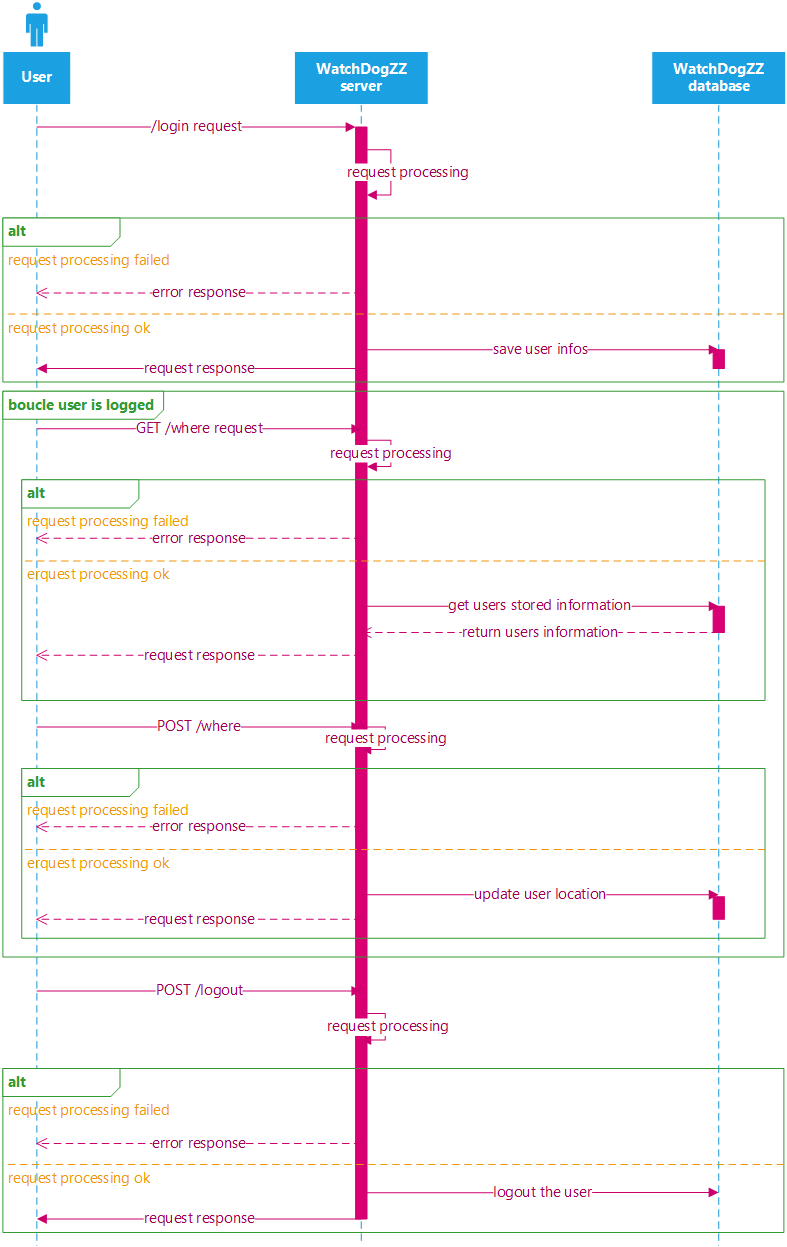
\includegraphics[height=0.99\textheight]{./img/server-requests.png}
    \caption{Diagramme de séquence des requêtes sur le service}
    \label{servicereq}
\end{figure}
